\chapter{Results} \label{results}
This chapter will encompass the result of the two ML models for NBRA prediction in Instagram and Flickr media objects as well as the evaluation of the ground truth data consisting of interviews and the passive observation statistic of NBRAs.
\section{Data-processing} \label{results_dataprocessing}
Table \ref{tab:data_reduction_values} provides an overview of the data-reduction for each used dataset as a result of the data-processing described in section \ref{data_processing} which consisted of:
\begin{itemize}
  \item in boundary check
  \item dominant authors exclusion
  \item bulk uploads
\end{itemize}

\begin{table}[h!]
\begin{center}
\caption{Listing of the applied thresholds and the resulting data-reduction of each dataset.}\vspace{1ex}
\label{tab:data_reduction_values}
\begin{tabular}{ccccc}\hline
dataset & excluded top authors & bulk threshold & input & output & data-reduction\\ \hline
Instagram Zug & 6 & 6 & 28'246 & 11'777 & 58.3\% \\
Instagram Zurich Uetliberg & 10 & 5 & 74'742 & 68'522 & 8.3\% \\
Instagram Zurich Dolder & 7 & 5 &  206'454 &  191'584 & 7.2\% \\
Flickr Zug & 12 & 7 &  14'236 &  3'790 & 73.4\% \\ 
Foursquare Zug & - & - & 405 & 378 & 6.7\% \\ \hline
\end{tabular}
\end{center}
\end{table}

The noticeably high data-reduction of the Flickr dataset was mostly due to large total upload numbers of a small share of users. Visible in figure \ref{img:dominant_users_flickr} are Flickr-users (authors) uploading up to 1'190 media objects since the launch of Flickr in the year 2004. As a result roughly 5'700 media objects were removed alone in the 'dominant user' data-processing step.

\begin{figure}[h!]
   \centering
   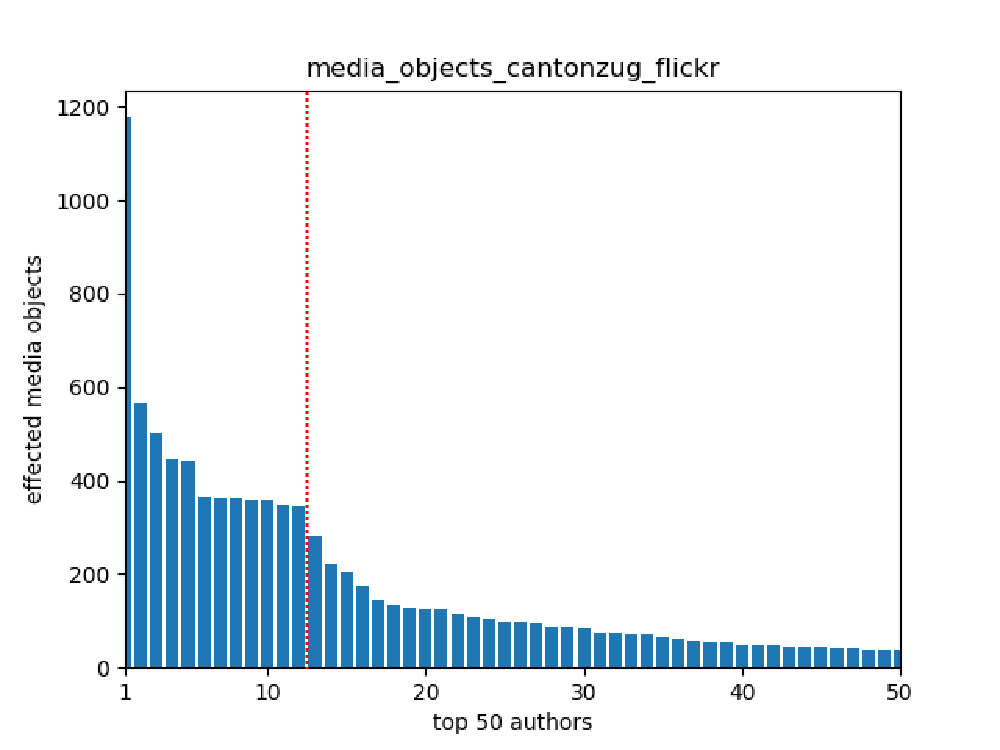
\includegraphics[width=0.75\textwidth]{img/cantonzug_flickr_top50_w_line}
   \caption{Overview of the uploaded media objects of the top 50 Flickr users since 2004 in the Canton of Zug. The top 12 users which account for roughly 5'700 media objects (left to the red line) were excluded from further data-analysis during the 'dominant' user data-processing step.}
   \label{img:dominant_users_flickr}
\end{figure}

As seen in figure \ref{img:bulk_uploads_flickr} an additional, roughly 3'000 Flickr media objects were removed in the 'bulk-upload' process. The y-values of that figure correspond to the potentially removed amount of media objects if a certain threshold on the x-axis is applied. The data visible in this graph only includes media objects which were not already excluded by preceding data-processing steps.

\begin{figure}[h!]
   \centering
   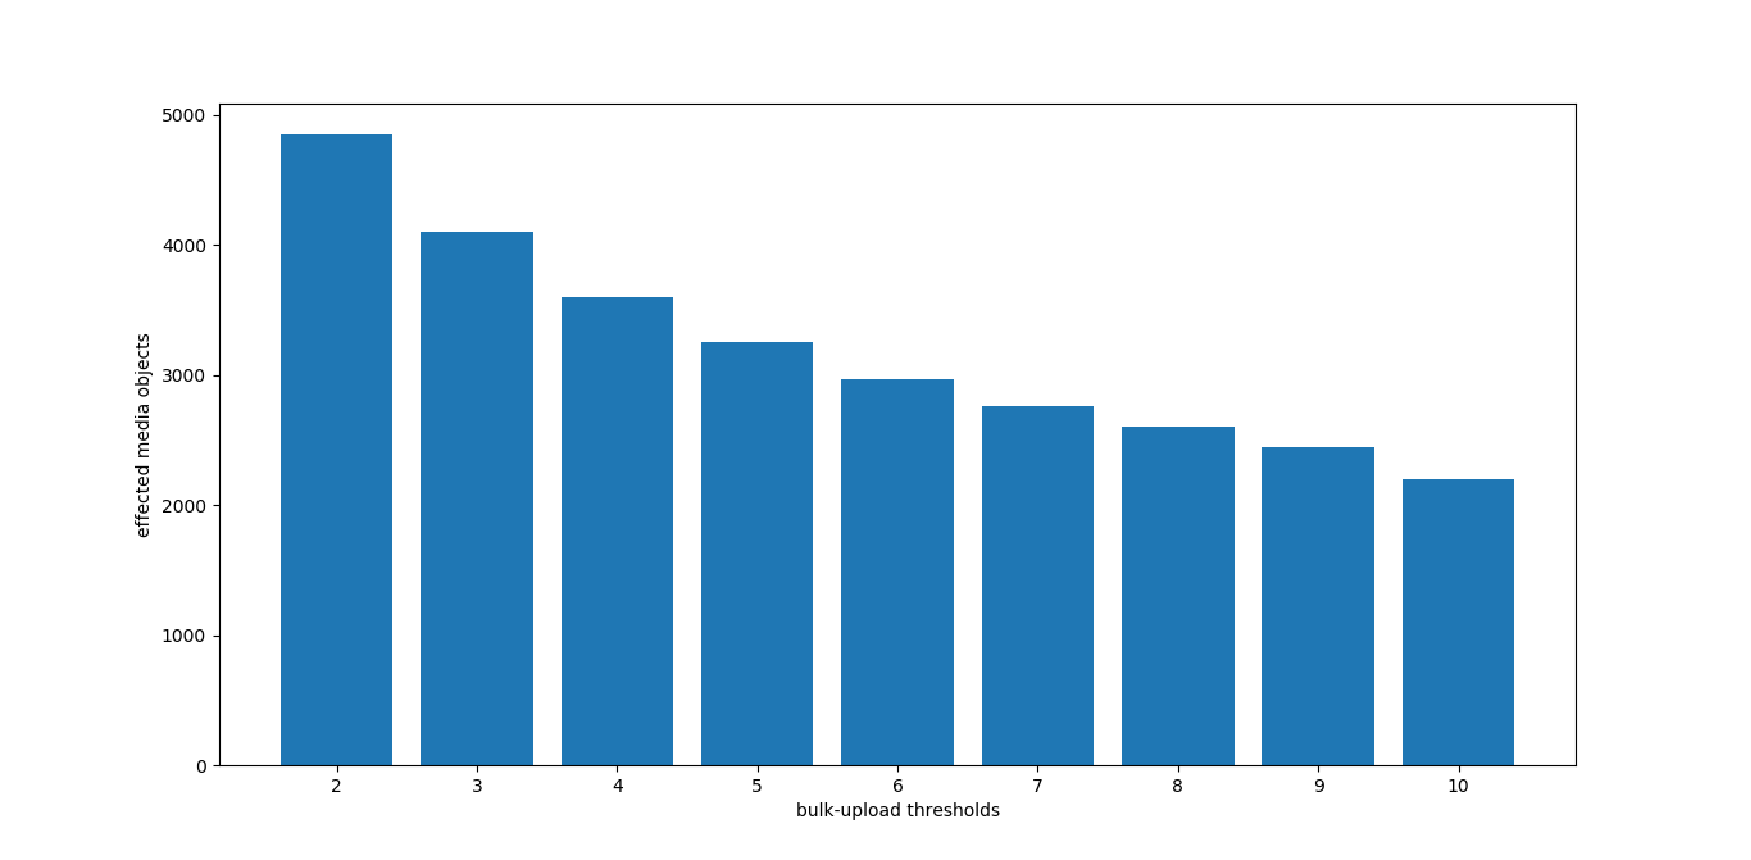
\includegraphics[width=0.75\textwidth]{img/cantonzug_flickr_bulkuploads_cropped.pdf}
   \caption{Shows the impact of different 'bulk-upload' thresholds on the Flickr dataset of the Canton of Zug}
   \label{img:bulk_uploads_flickr}
\end{figure}

Similar graphs to figure \ref{img:dominant_users_flickr} and \ref{img:bulk_uploads_flickr} were created for all the datasets. The functioned as a basis for manually declaring the thresholds visible in \ref{tab:data_reduction_values}. 

\section{Models} \label{results_models}
The performance results of the two in section \ref{ml_model} introduced models will subsequently be presented. These models were both solely trained on the Instagram Zurich Dolder and Instagram Zurich Uetliberg datasets included in the database table: \texttt{media\_objects\_trainingdata\_instagram} (database overview visible in figure \ref{database_setup}). For each model the Random Forest classifier and the linearSVC fitting algorithm were independently tested. The hyperparameters were tuned to yield the best possible 10-fold cross-validated F1-score averaged over all classes excluding the None-class. The training data was consistently split into 75\% for training and 25\% for testing. Simultaneously, the effect of including different amounts of the None-class training data media objects during model fitting were also investigated. These values ranged from 500 to 6'500 with steps of 500.\\
These models were then used to predict the NBRAs contained in the media objects of the Instagram database table: \texttt{media\_objects\_unionzug\_instagram} and the \\Flickr database table: \texttt{media\_objects\_cantonzug\_flickr}\\
Each model performed two separate predictions on each of the above mentioned datasets which differed in the final text-string composition that was parsed for prediction. One time the final text-string was constructed by concatenating the processed text-data and the image labels of a given media object. The second time the final text-string only contained the processed text-data.\\
\newline
\texttt{Remark:} The entire data presented in the following subsections is available on the enclosed CD. This includes the actual M1 and M2 dump files, tuning and cross-validation logs as well as the performance graphs (see chapter \ref{CD_content}).

\subsection{Model 1: untrained on image labels}
The first model (M1) that was trained exclusively on processed user generated text-data. Therefore, it did not include any image content information.

\subsubsection{M1 - Random Forest}
The model tuning according to the parameter grid visible in figure \ref{coderandomForestparameters} resulted in the following best performing hyperparameter constellation:

\begin{table}[h!]
\begin{center}
\caption{Best M1 hyperparameter setting for the Random Forest algorithm. The parameter descriptions can be found in section \ref{model_setup}}\vspace{1ex}
\label{tab:m1_randomForest_bestParams}
\begin{tabular}{ccccc}\hline
k & max\_depth & min\_df & ngram\_range & none\_objects \\ \hline
all & None (no restriction) & 11 & (1, 1) & 3'500 \\ \hline
\end{tabular}
\end{center}
\end{table}

The hyperparameter setting visible in table \ref{tab:m1_randomForest_bestParams} allowed for the best model performance with a resulting number of \textbf{727 features}. All scores were rounded to three decimal places and were calculated with the \textit{scikit-learn} 'weighted' parameter. 'F1' refers to the weighted average across all classes whereas the 'F1 without None-class' refers to the weighted average across all classes except the None-class.

\begin{table}[h!]
\begin{center}
\caption{M1 Random Forest performance scores during testing (except accuracy train)}\vspace{1ex}
\label{tab:m1_randomForest_bestscores}
\begin{tabular}{cccccc}\hline
Accuracy train & Accuracy test & Precision & Recall & F1 & F1 (without None-class)\\ \hline
0.999 & 0.941 & 0.941 & 0.941 & 0.936 & 0.757 \\ \hline
\end{tabular}
\end{center}
\end{table}

\subsubsection{M1 - LinearSVC}
The model tuning with the parameter grid visible in figure \ref{codelinearsvcparameters} resulted in the following best performing hyperparameter constellation:

\begin{table}[h!]
\begin{center}
\caption{Best M1 hyperparameter setting for the linearSVC algorithm. The parameter descriptions can be found in section \ref{model_setup}}\vspace{1ex}
\label{tab:m1_linearSVC_bestParams}
\begin{tabular}{llccc}\hline
k & C & min\_df & ngram\_range & none\_objects \\ \hline
all & 1 & 12 & (1, 1) & 3'000 \\ \hline
\end{tabular}
\end{center}
\end{table}

This hyperparameter setting visible in the table \ref{tab:m1_linearSVC_bestParams} allowed for the best model performance with a resulting number of \textbf{626 features}. All scores were rounded to three decimal places. 'F1' refers to the weighted average across all classes whereas 'F1 without None-class' refers to the weighted average across all classes except the None-class.

\begin{table}[h!]
\begin{center}
\caption{M1 linearSVC performance scores during testing (except accuracy train)}\vspace{1ex}
\label{tab:m1_linearSVC_bestscores}
\begin{tabular}{cccccc}\hline
Accuracy train & Accuracy test & Precision & Recall & F1 & F1 (without None-class)\\ \hline
0.983 & 0.937 & 0.937 & 0.937 & 0.937 & 0.870 \\ \hline
\end{tabular}
\end{center}
\end{table}

\subsection{Model 2: trained on image labels and text-data}
The second model (M2) was trained on the Google Cloud Vision API image labels extracted from the media objects images and the processed user generated text-data.

\subsubsection{M2 - Random Forest}
The model tuning with the parameter grid visible in figure \ref{coderandomForestparameters} resulted in the following best performing hyperparameter constellation:\\

\begin{table}[h!]
\begin{center}
\caption{Best M2 hyperparameter setting for the Random Forest algorithm. The parameter descriptions can be found in section \ref{model_setup}}\vspace{1ex}
\label{tab:m2_randomForest_bestParams}
\begin{tabular}{llccc}\hline
k & max\_depth & min\_df & ngram\_range & none\_objects \\ \hline
all & None (no restriction) & 14 & (1, 1) & 400 \\ \hline
\end{tabular}
\end{center}
\end{table}

This hyperparameter setting visible in the table \ref{tab:m2_randomForest_bestParams} allowed for the best model performance with a resulting number of \textbf{324 features}. All scores were rounded to three decimal places and were calculated with the \textit{scikit-learn} 'weighted' parameter. 'F1' refers to the weighted average across all classes whereas 'F1 without None-class' refers to the weighted average across all classes except the None-class.

\begin{table}[h!]
\begin{center}
\caption{M2 Random Forest performance scores during testing (except accuracy train)}\vspace{1ex}
\label{tab:m2_randomForest_bestscores}
\begin{tabular}{cccccc}\hline
Accuracy train & Accuracy test & Precision & Recall & F1 & F1 (without None-class)\\ \hline
0.998 & 0.892 & 0.903 & 0.901 & 0.892 & \textbf{0.745}\\ \hline
\end{tabular}
\end{center}
\end{table}

\subsubsection{M2 - LinearSVC}
The model tuning with the parameter grid visible in figure \ref{codelinearsvcparameters} resulted in the following best performing hyperparameter constellation:

\begin{table}[h!]
\begin{center}
\caption{Best M2 hyperparameter setting for the linearSVC algorithm. The parameter descriptions can be found in section \ref{model_setup}}\vspace{1ex}
\label{tab:m2_linearSVC_bestParams}
\begin{tabular}{llccc}\hline
k & C & min\_df & ngram\_range & none\_objects \\ \hline
all & 1 & 7 & (1, 1) & 700 \\ \hline
\end{tabular}
\end{center}
\end{table}

This hyperparameter setting visible in the table \ref{tab:m2_linearSVC_bestParams} allowed for the best model performance with a resulting number of \textbf{775 features}. All scores were rounded to three decimal places. 'F1' refers to the weighted average across all classes whereas 'F1 without None-class' refers to the weighted average across all classes except the None-class.

\begin{table}[h!]
\begin{center}
\caption{M2 linearSVC performance scores during testing (except accuracy train)}\vspace{1ex}
\label{tab:m2_linearSVC_bestscores}
\begin{tabular}{cccccc}\hline
Accuracy train & Accuracy test & Precision & Recall & F1 & F1 (without None-class)\\ \hline
0.993 & 0.882 & 0.883 & 0.886 & 0.882 & \textbf{0.835} \\ \hline
\end{tabular}
\end{center}
\end{table}

\subsubsection{Best features}
Both linearSVC models consist of more than 600 features. The information gain or coefficient magnitude on the other hand that individual features provide differs. Figure \ref{fig:M2_top40_features_biking} visualises the 40 most predictive features that support the prediction of the class 'biking' (blue) as well as the top 40 features that indicate the opposite (red). Similar figures for the remaining classifications 'walking', 'hiking', 'jogging', 'dog walking', 'horse riding', 'picnic' and 'None' can be found in Appendix \ref{M2_top_features}. 
\begin{figure}[h!]
   \centering
   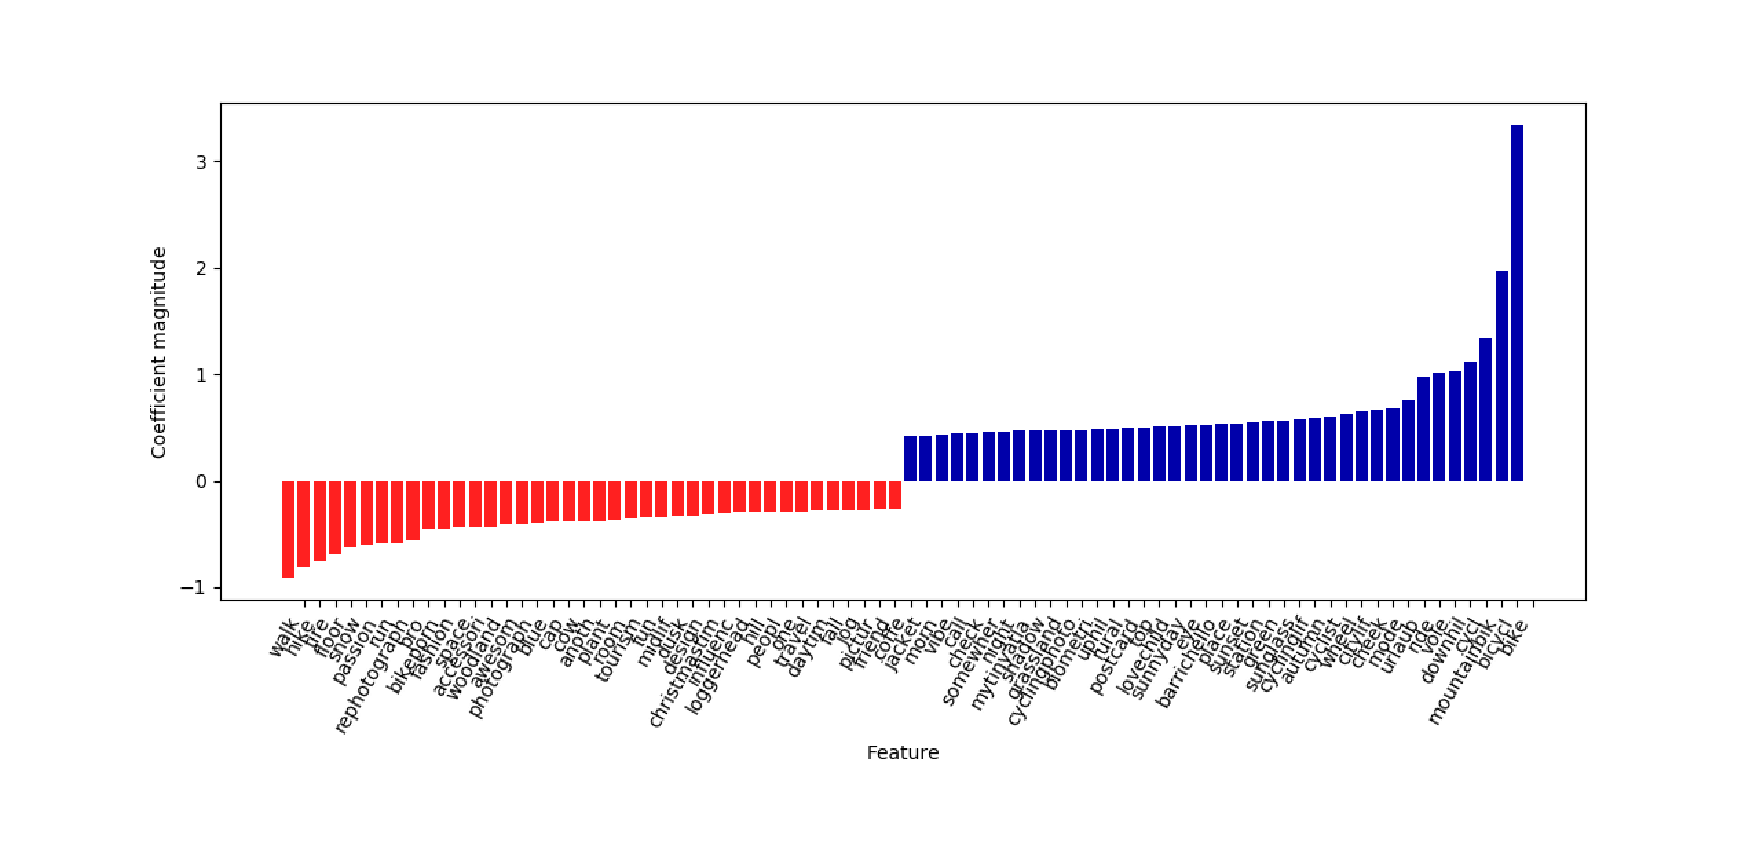
\includegraphics[width=\textwidth]{img/m2_top_40_features_Biking_cropped.pdf}
   \caption{The top 80 most predictive M2-features of the class 'biking'. Blue features are word-tokens which supports the presence of the corresponding classification. Red features support the opposite. The graphic was created with the \textit{mglearn} Python library provided by \textcite{Guido2016}}
   \label{fig:M2_top40_features_biking}
\end{figure}

\subsection{Model comparison}
The above presented models will subsequently be thoroughly compared in terms of classification specific aspects, hyperparameter behaviour and performance on unseen data (data the models were not trained on). 

\subsubsection{Hyperparameter interaction}
The effect of different \textit{ngram\_range} settings in combination with varying \textit{C} values of the linearSVC fitting algorithm is illustrated in the heatmaps of figure \ref{fig:heatmaps} for M1 and M2 respectively. The red circles mark the combination with the highest F1-score which corresponds to the best hyperparameter setting of the respective models (see M1 - table \ref{tab:m1_linearSVC_bestParams} and M2 - table \ref{tab:m2_linearSVC_bestParams}). It becomes apparent that the (2, 2) \textit{ngram\_range} as well as the \textit{C} value 0.01 underperform across the board. The F1-scores in the heatmaps are not completely identical to the values found in the corresponding model performance tables \ref{tab:m1_linearSVC_bestscores} (M1) and \ref{tab:m2_linearSVC_bestscores} (M2). This variation is due to randomisation effects of the None media object selection from the database as well as from the model train and test splits (this is partly taken care of by cross-validation).\\

\begin{figure}[h!]
 \begin{subfigure}{0.5\textwidth}
   \centering
   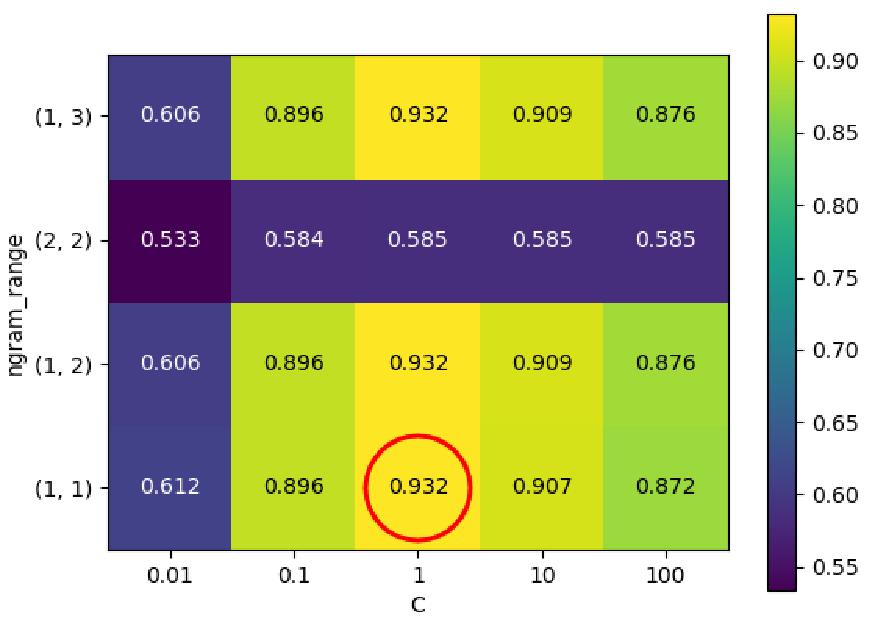
\includegraphics[width=0.9\linewidth]{img/m1_F1_ngram_C_heatmap_w_Circle.pdf}
   \caption{M1 linearSVC}
   \label{fig:m1_heatmap}
\end{subfigure}
\begin{subfigure}{0.5\textwidth}
   \centering
   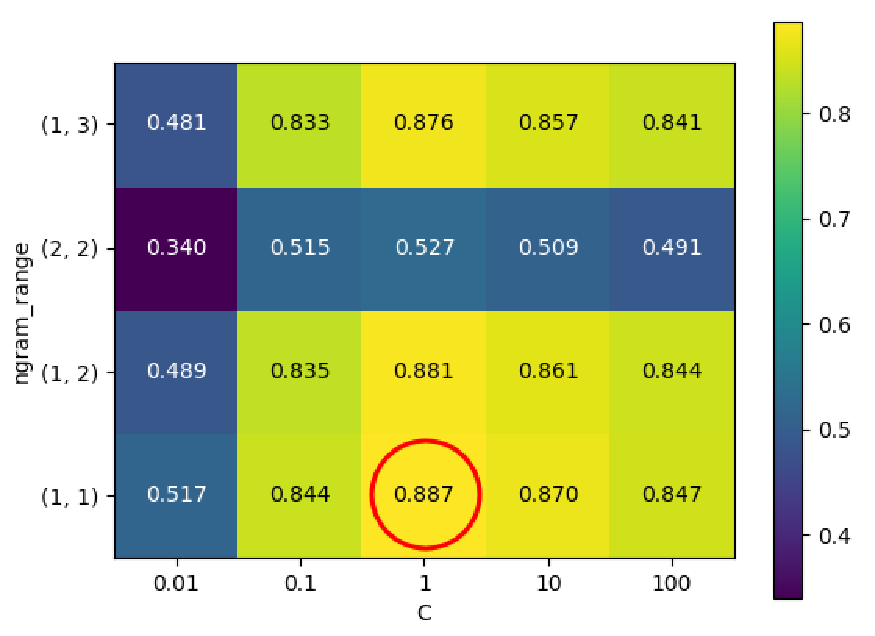
\includegraphics[width=0.9\linewidth]{img/m2_ngram_C_heatmap_new_w_circle.pdf}
   \caption{M2 linearSVC}
   \label{fig:m2_heatmap}
 \end{subfigure}
\caption{These heatmaps shows cross-validated F1-scores of different combinations of the hyperparameters \textit{ngram\_range} and \textit{C} for the linearSVC model M1 (a) and M2 (b). These graphs were created with the Python library \textit{mglearn} from \textcite{Guido2016}}
\label{fig:heatmaps}
\end{figure}

\texttt{Remark:} If different hyperparameter settings produce the same model performance (F1-score) than the setting which produces fewer features is prioritised due to better generalisation and regularisation capabilities. Regarding figure \ref{fig:m1_heatmap} for instance the \textit{ngram\_range} setting of either (1, 1), (1, 2) or (1, 3) in combination with \textit{C} = 1 all produce a F1-score of 0.932. (1, 1) has been chosen as best hyperparameter configuration due to the lowest feature count.

\subsubsection{Classification specific F1-scores}
As already seen above M1 performed on the test set with an 10-fold cross-validated F1-score excluding the None-class of \textbf{0.870} compared to \textbf{0.835} of M2. Figure \ref{fig:m1_m2_class_f1_scores} gives more insight on the classification specific model performances. The worst performances are recorded for both Random Forest classifiers. Also the M2 linearSVC picnic class sticks out with a score of 0.48. The actual performance and generalisation potential of both model on 'unseen data' is presented further down.
\begin{figure}[h!]
   \centering
   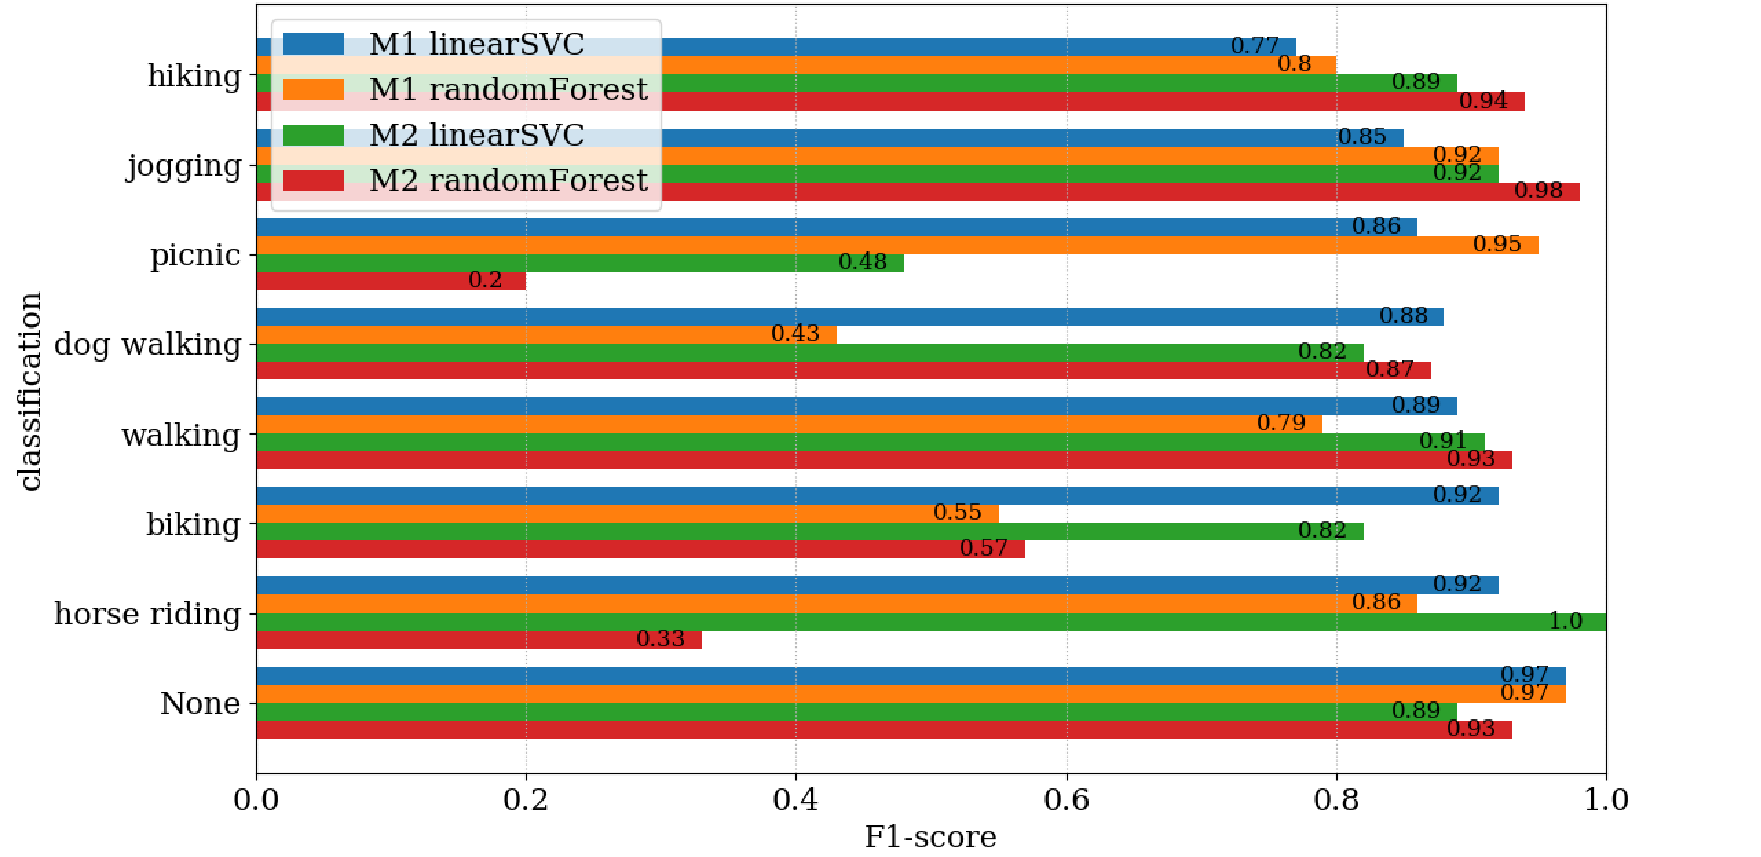
\includegraphics[width=\textwidth]{img/m1_m2_class_f1_scores_bigger_font.pdf}
   \caption{Overview of the classification specific 10-fold cross-validated F1-scores of the linearSVC and Random Forest fitting algorithm of M1 and M2}
   \label{fig:m1_m2_class_f1_scores}
\end{figure}

\subsubsection{Final model scores}
In the end both models were trained on the entire training dataset which resulted in the following final performance scores visible in table \ref{tab:m1_m2_linearSVC_final_scores}. This step is important to generate a finalised model that is eventually trained on as much training data as possible. Keeping a data aside for model testing is no longer necessary because the most well performing hyperparameter configuration is already determined.\\
It can be noted at this point that the best M1 and M2 performance yielded similar feature counts during testing (626 and 775 respectively) as well as after training it on the entire dataset (845 and 958 respectively). Also, contradicting to the already presented model performances during model-tuning M2 now performs slightly better than M1. Possible reasons for this observation will be discussed in the section \ref{disussion_model_performance}.

\begin{table}[h]
\begin{center}
\caption{linearSVC 10-fold cross-validated final performance scores of M1 and M2 while being fitted according to the entire training dataset available.}\vspace{1ex}
\label{tab:m1_m2_linearSVC_final_scores}
\begin{tabular}{cccccc}\hline
Model & Accuracy & Precision & Recall & F1 & F1 (without None-class) & Features\\ \hline
M1 & 0.984 & 0.984 & 0.984 & 0.984 & 0.967 & 845\\
M2 & 0.991 & 0.991 & 0.991 & 0.991 & 0.993 & 958\\ \hline
\end{tabular}
\end{center}
\end{table}

\subsubsection{Precision on unseen data} \label{precision_unseen_data}
This section will present the model performances on new data. All Instagram and Flickr media objects of the Canton of Zug on which these results are based were excluded from the M1 and M2 model training.\\
Two separate predictions per model were performed on the media objects contained in the following two database-tables (database overview see section \ref{database_setup}):

\begin{itemize}
    \item \texttt{media\_objects\_unionzug\_instagram} \item \texttt{media\_objects\_cantonzug\_flickr}
\end{itemize}

One time the final text-string provided for the prediction was constructed by concatenating the processed text-data and the image labels of a given media object. The second time the final text-string only contained the processed text-data.\\

The model performance evaluation was done manually by the author. 100 media objects (if available) per class, per prediction-mode and per model were evaluated for True Positive (TP) or False Positive (FP) predictions. Only the model precision can be calculated with this information. An estimate for the recall over all classes was made based on the share of media objects that were correctly classified (except the None-class) in relation to the total amount of media objects present. In other words, how many media objects that actually contained NBRAs were also identified as such? This information is important because e.g. a model with 95\% precision that only identifies 20\% of media objects containing NBRAs is still not practical. This approximation was calculated in the following way:

\begin{ceqn}
\begin{align}
\label{equation_share_TP}
\frac{\sum_{class=1}^{7}(precision_{class}  * n^{total}_{class})}{n^{total}_{dataset}} * 100
\end{align}
\end{ceqn}

where the class-specific model precision (\textit{precision}\textsubscript{class}) is based on the manual evaluation of 100 media objects of that class which can be a subset of the total amount of predicted media objects of that class by the model.

\paragraph*{Model 1}
The best M1 precision of \textbf{0.714} was recorded for the media objects of the social media platform Flickr while the parsed text-string excluded image labels (see table \ref{tab:m1_actual_precision}). Predicting new data without image labels across both social media platforms yields accordingly an average precision score of \textbf{0.711}.\\
While the M1 precision differences between the two social media platforms Instagram and Flickr were not significant on a 5\% level, the recorded differences between the inclusion and exclusion of image labels were significant.

\begin{table}[h!]
\begin{center}
\caption{M1 precision on unseen data}\vspace{1ex}
\label{tab:m1_actual_precision}
\begin{tabular}{c|cc?cc}\hline
platform & +image labels & -image labels & $\bar{x}$ & ratio\\ \hline
Instagram & 0.664 & 0.708 & 0.686 & 0.938\\ %0.664 & 0.732 & 0.698 & 0.907
Flickr & 0.634 & 0.714 & 0.674 & 0.888\\ %0.634 & 0.764 & 0.699 & 0.830
\Xhline{2\arrayrulewidth}
$\bar{x}$ & 0.649 & 0.711 \\ %& 0.649 & 0.748 
%\cline{1-3}
ratio & 1.047 & 0.992    %1.047 & 0.958 
\end{tabular}
\end{center}
\end{table}

The incorporation of image labels into the text-string results in an increase of overall and true positive predictions for both social media platforms (see table \ref{tab:m1_actual_recall}).
In the case of Instagram the inclusion and exclusion of image labels results in a total of \textbf{668} and \textbf{384} NBRA-identifications which corresponds to 5.67\% and 3.26\% respectively of the 11'777 media objects in the database table \texttt{media\_objects\_unionzug\_instagram}.
In the case of Flickr the inclusion and exclusion of image labels results in a total of \textbf{273} and \textbf{67} NBRA-identifications which corresponds to 4.25\% and 1.77\% respectively of the 3'790 media objects in the database table \texttt{media\_objects\_cantonzug\_flickr}.\\
Therefore, the best performing final text-string format which excludes image labels results in a total of \textbf{451} (extrapolation based on the calculated precision on 100 media objects per class) true positive NBRA media objects across both social media platforms. 

\begin{table}[h!]
\begin{center}
\caption{Share of correctly classified NBRA media objects by M1 (except the None-class) in relation to the entire dataset (according to listing \ref{equation_share_TP})}\vspace{1ex}
\label{tab:m1_actual_recall}
\begin{tabular}{ccc?cc}\hline
platform & +image labels & -image labels & $\bar{x}$ & ratio\\ \hline
Instagram & 5.67\% & 3.26\% & 4.47\% & 1.74\\
Flickr & 4.25\% & 1.77\% & 3.01\% & 2.40\\
\Xhline{2\arrayrulewidth}
$\bar{x}$ & 4.96\% & 2.52\% \\
ratio & 1.33 & 1.84 
\end{tabular}
\end{center}
\end{table}

\paragraph*{Model 2}
The best M2 precision of \textbf{0.776} was recorded for the media objects of the social media platform Instagram while the parsed text-string included image labels (see table \ref{tab:m2_actual_precision}). Predicting new data with image labels across both social media platforms yields accordingly an average model performance of \textbf{0.749}.\\
While the M2 precision differences between the two social media platforms Instagram and Flickr were not significant on a 5\% level, the recorded differences between the inclusion and exclusion of image labels were significant.\\


\begin{table}[h!]
\begin{center}
\caption{M2 precision on unseen data}\vspace{1ex}
\label{tab:m2_actual_precision}
\begin{tabular}{ccc?cc}\hline
platform & +image labels & -image labels & $\bar{x}$ & ratio\\ \hline
Instagram & 0.776 & 0.691 & 0.734 & 1.123\\
Flickr & 0.721 & 0.753 & 0.737 & 0.958\\
\Xhline{2\arrayrulewidth}
$\bar{x}$ & 0.749 & 0.722\\
ratio & 1.076 & 0.918   
\end{tabular}
\end{center}
\end{table}

The incorporation of image labels into the final text-string results in a significant increase of overall and true positive predictions for both social media platforms (see table \ref{tab:m2_actual_recall}).
In the case of Instagram the inclusion and exclusion of image labels results in a total of \textbf{710} and \textbf{137} NBRA-identifications which corresponds to 6.03\% and 3.63\% respectively of the 11'777 media objects in the database table \texttt{media\_objects\_unionzug\_instagram}. In the case of Flickr the inclusion and exclusion of image labels results in a total of \textbf{227} and \textbf{82} NBRA-identifications which corresponds to 5.99\% and 2.16\% respectively of the 3'790 media objects in the database table \texttt{media\_objects\_cantonzug\_flickr}.\\
Therefore, the best performing final text-string format which includes image labels results in a total of \textbf{937} (extrapolation based on the calculated precision on 100 media objects per class) true positive NBRA media objects across both social media platforms. 

\begin{table}[h!]
\begin{center}
\caption{Share of correctly classified NBRA media objects by M2 (except the None-class) in relation to the entire dataset (according to listing \ref{equation_share_TP})}\vspace{1ex}
\label{tab:m2_actual_recall}
\begin{tabular}{ccc?cc}\hline
platform & +image labels & -image labels & $\bar{x}$ & ratio\\ \hline
Instagram & 6.03\% & 3.63\% & 4.83\% & 1.66\\
Flickr & 5.99\% & 2.16\% & 4.08\% & 2.77\\
\Xhline{2\arrayrulewidth}
$\bar{x}$ & 6.01\% & 2.90\% \\
ratio & 1.00 & 1.68 
\end{tabular}
\end{center}
\end{table}

\paragraph*{Summary}
M1 and M2 showed both the best performance if the parsed data for prediction (final text-string) was in the form the model was originally trained.\\
The model precision was less dependant on the social media platform the media objects originated from but rather if image labels were parsed or not.\\
The best observed precision of M2 with \textbf{0.776} (platform average: 0.749) was only slightly better than the \textbf{0.714} of M1 (platform average: 0.711). Strong differences were registered in the percentage of correctly classified media objects in relation to the entire dataset which lay at \textbf{6.01\%} for M2 but only at \textbf{2.52\%} for M1.
M2 with a slightly higher precision yielded (937-451=)486 more true positive NBRA-predictions than M1 which resolves to an \textbf{increase by factor two}. Therefore, M2 predicted less False Negatives (FN) which concludes that M2 also possess a higher recall score than M1 and generalises better on new data.

\section{Media object languages}
One assumption that was made earlier stated that the training data from Zurich and the media objects from Zug share a similar written language by their author base. This would legitimise the usage of training data that did not originate from the same region as the region the model would later be applied to.\\
To investigate on that assumption the five actively detected Instagram media object languages of both regions were compared (see figure \ref{fig:det_languages}) with a paired two sample t-test for means. The result showed on a significance level of 5\% that the probability that T is smaller or equal to t is 0.56 and therefore smaller than t\textsubscript{crit} of 2.78. Therefore, the null-hypothesis \textit{H\textsubscript{0}} (no difference present) cannot be rejected and the written languages of both areas are with high certainty of similar composition.

\begin{figure}[h!]
   \centering
   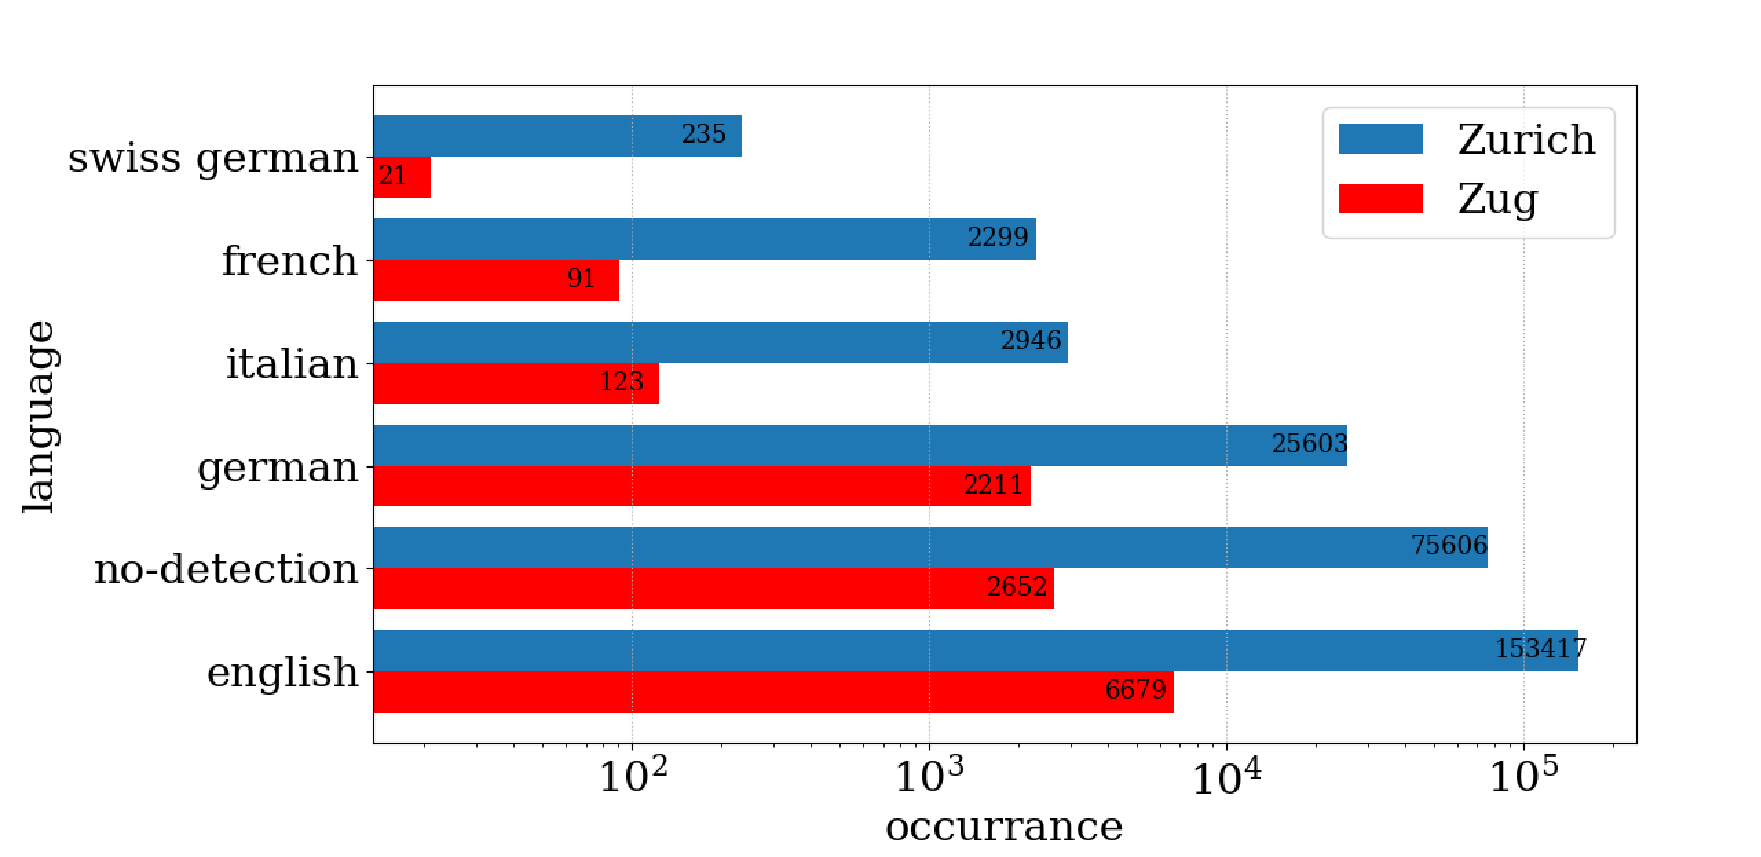
\includegraphics[width=\textwidth]{img/det_languages_bigger_font.pdf}
   \caption{Comparison between detected languages of Instagram media objects originating from the Canton of Zug and Zurich}
   \label{fig:det_languages}
\end{figure}

\texttt{Remark:} Often times hashtags remain written in English due to their comprehensive meaning and purpose to connect media objects of similar content. Due to the big share hashtags normally have on the entire text corpus the language detection tends to identify a media object language as English above others.

\section{Ground truth evaluation}
The following subsections will cover the results from the \textit{in-situ} ground truthing through passive observations and the 52 interviews over the three different locations 'Br\"uggli', 'R\"ossliwiese' and 'Schattenw\"aldli' (see figure \ref{fig:locations_ground_truthing}) in the research area. \\

\newline

\texttt{Remark:} The entire data presented in the following subsections is available on the enclosed CD to this thesis. This includes the actual transcript-data from the passive observation and the interviews (see chapter \ref{CD_content}).

\subsection{Passive observation analysis}
The passive NBRA-observation was performed by an assistant of the author. The thereby collected data is visible in figure \ref{fig:passive_observation} and shows the recorded NBRAs based on location sorted from left to right by decreasing observation frequency. Walking and hiking were by far the most recorded classes which corresponds to the interviews results visible in figure \ref{fig:interview_activities}. These two classes were merged due to differentiation difficulties just by observation and the demanded recording speed. 'Biking' follows second with a strong signal in the location 'Br\"uggli' and no occurrence at 'R\"ossliwiese'. Third is 'jogging' shortly followed by 'dog walking' which have roughly the same occurrence frequency distribution across all three locations.

\begin{figure}[h!]
   \centering
   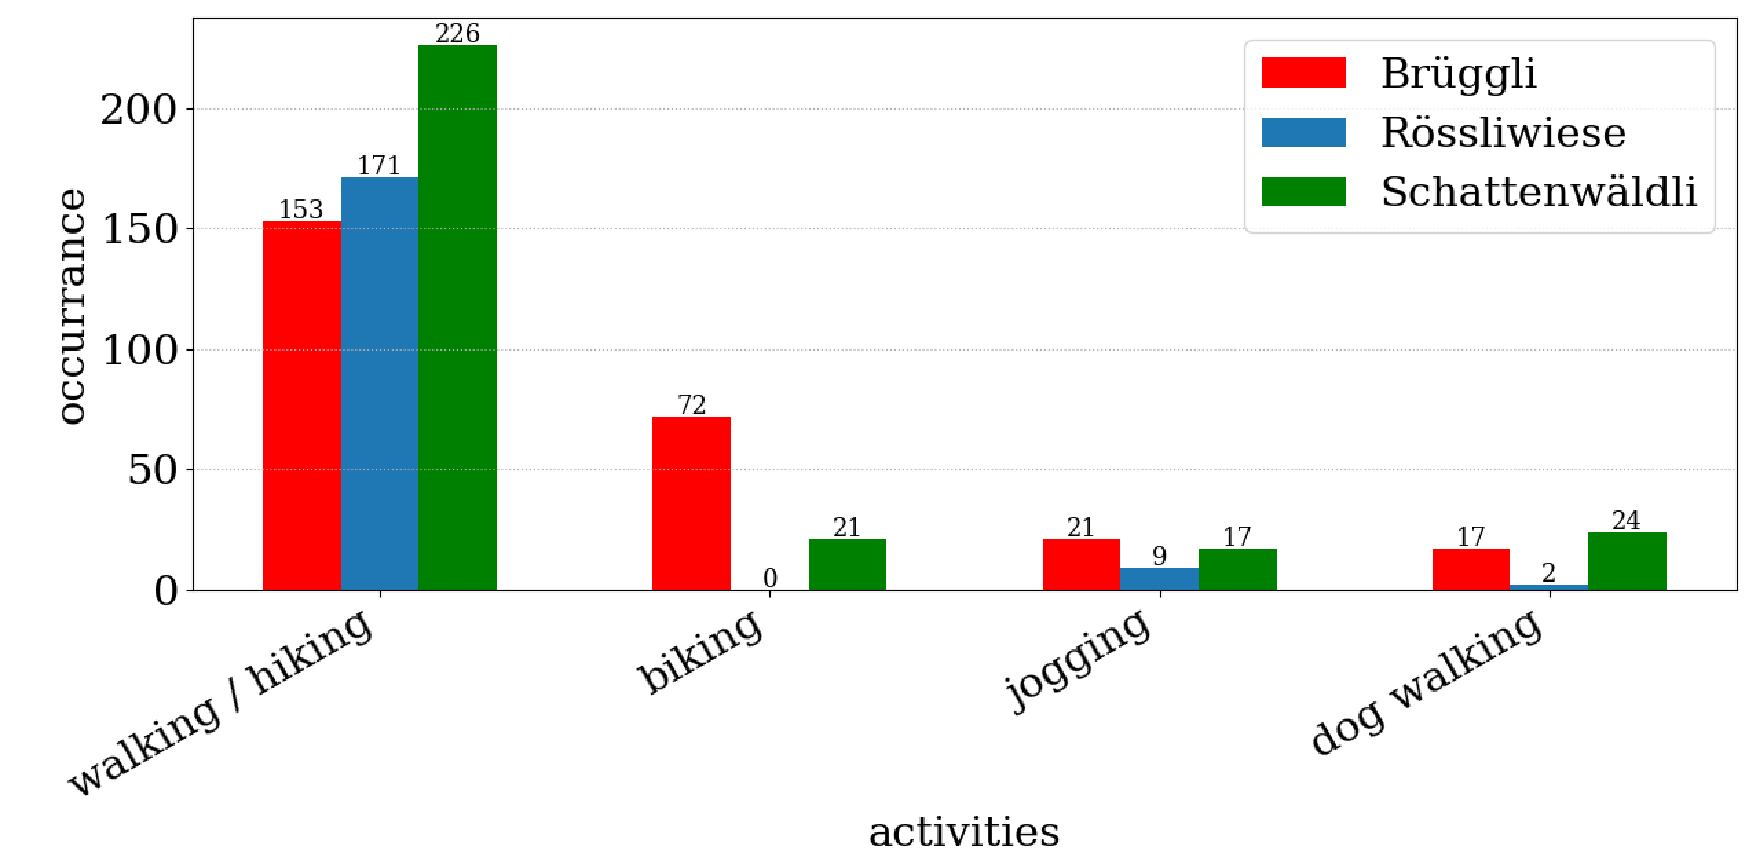
\includegraphics[width=\textwidth]{img/passive_observations.pdf}
   \caption{NBRA-occurrence according to the passive observation performed in the three locations listed in the legend}
   \label{fig:passive_observation}
\end{figure}

\subsection{Interview analysis}

\subsubsection{Visitation motivations}
The top eight motivations or reasons the interviewees mentioned why they visited a given location are displayed in figure \ref{fig:interview_visitation_motivation} sorted from left to right in descending order. According to the results plays \textit{geographic closeness} a dominant role how people choose their location for recreation. If a lake was present it was also frequently mentioned as a strong driver that attracts people for NBRAs. The term \textit{sport} was solely mentioned for the location 'Schattenw\"aldli', the terms \textit{shopping}, \textit{low traffic} and \textit{sunset} exclusively for the location 'R\"ossliwiese' and the term \textit{topography} for the location 'Br\"uggli'.

\begin{figure}[h!]
   \centering
   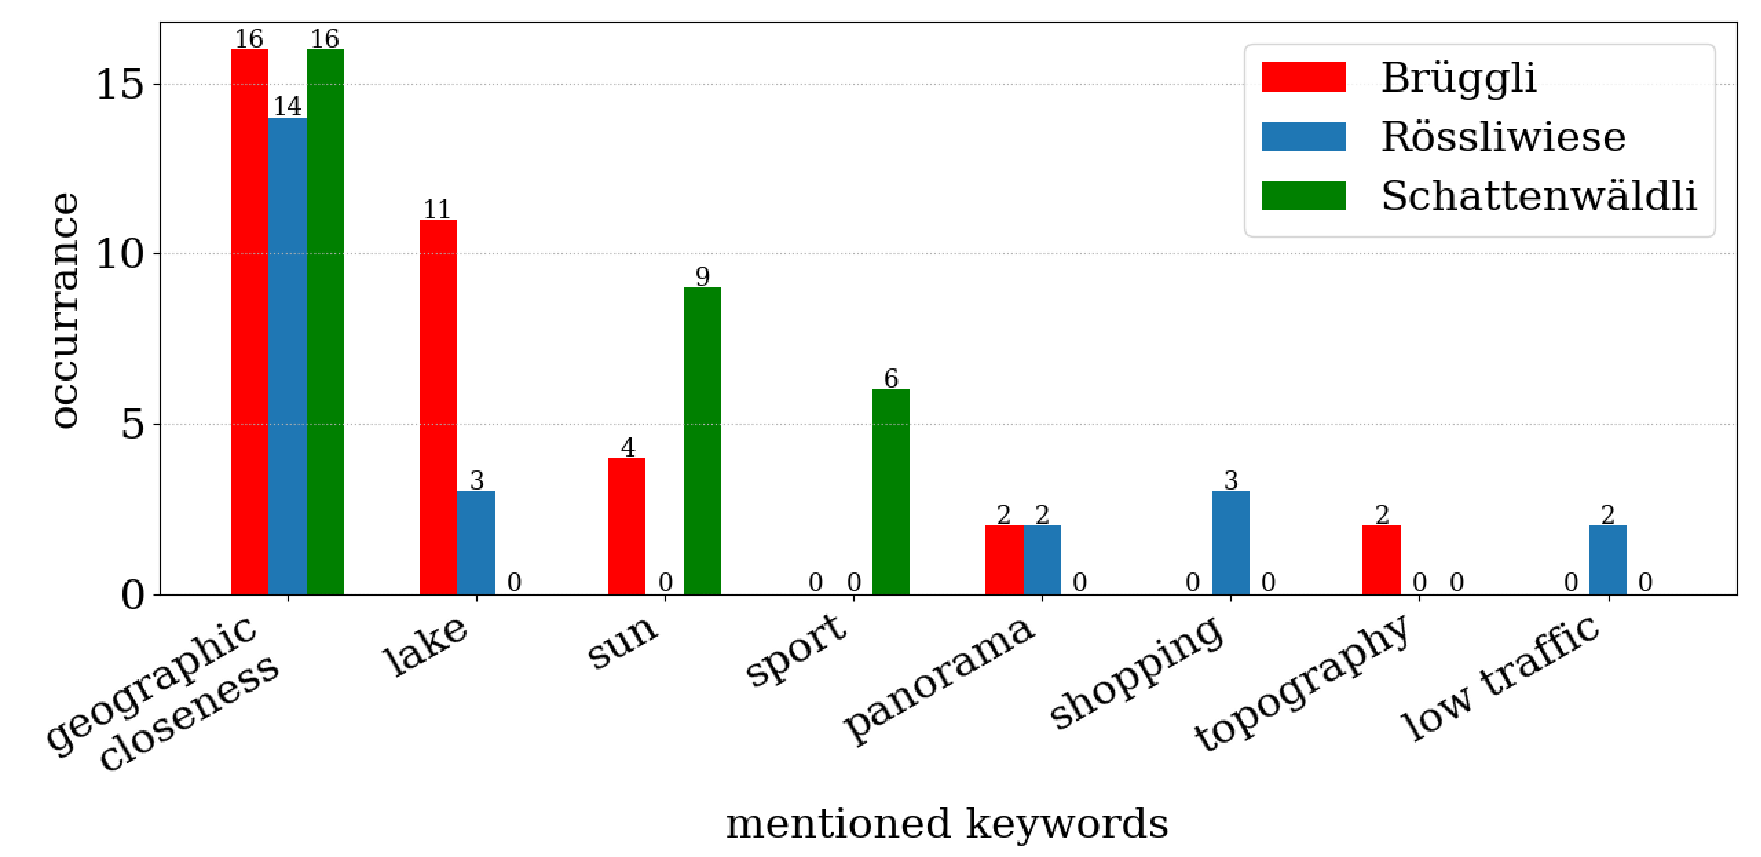
\includegraphics[width=\textwidth]{img/interview_keywords.pdf}
   \caption{Frequency of drivers mentioned by 52 interviewees for visiting one of the three locations listed in the legend.}
   \label{fig:interview_visitation_motivation}
\end{figure}

\subsubsection{Recorded NBRAs}
Figure \ref{fig:interview_activities} corresponds to figure \ref{fig:passive_observation} and shows similarly the performed NBRAs. This time the descriptive term came from the interviewees themselves which explains why the differentiation between the classes 'walking' and 'hiking' is again established. 'Walking' still holds the biggest share across all three locations. 'Biking' follows again second and was recorded everywhere but in the location 'R\"ossliwiese' to which 'relaxing' was exclusive. Third comes 'hiking' which was only found on the mountain location 'Schattenw\"aldli'. The NBRA 'swimming' was not actively performed at the time of the interviews but it was instead mentioned by the interviewees as a regular summer activity at the location 'Br\"uggli'.

\begin{figure}[h!]
   \centering
   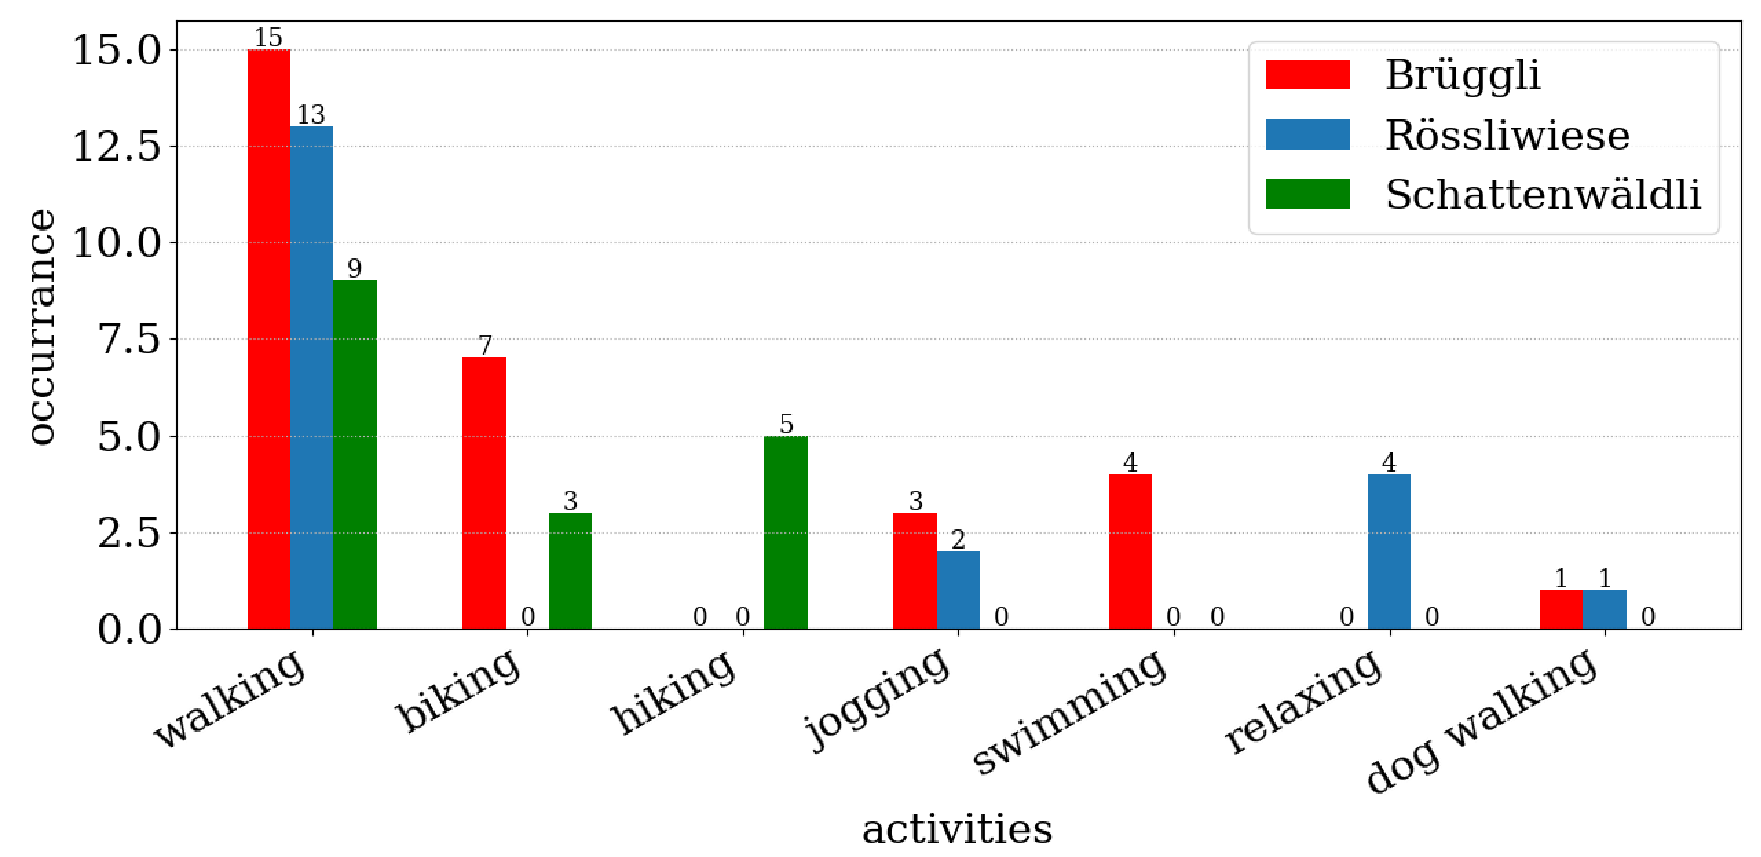
\includegraphics[width=\textwidth]{img/interview_activities.pdf}
   \caption{NBRA-occurrence according to the 52 performed interviews in the three locations listed in the legend}
   \label{fig:interview_activities}
\end{figure}

\subsubsection{Popularity of social media platforms }
One main part of the interviews next to the information gain related to the performed NBRAs was dedicated to the interviewee's social media usage and engagement. Figure \ref{fig:interview_SMP} visualises the recorded occurrences where interviewees confirmed having an account on one of the given social media platforms. Instagram and Facebook are by far the most widespread social media platforms that were registered. LinkedIn follows third with less than half of the mentions of first or second place. Many interviewees mentioned the (sometimes forced) requirement of a LinkedIn account for their professional life. A surprisingly low occurrence is registered for Twitter. STRAVA through being a specialised social media platform was only mentioned once. Interestingly Flickr was not mentioned once during all 52 interviews.

\begin{figure}[h!]
   \centering
   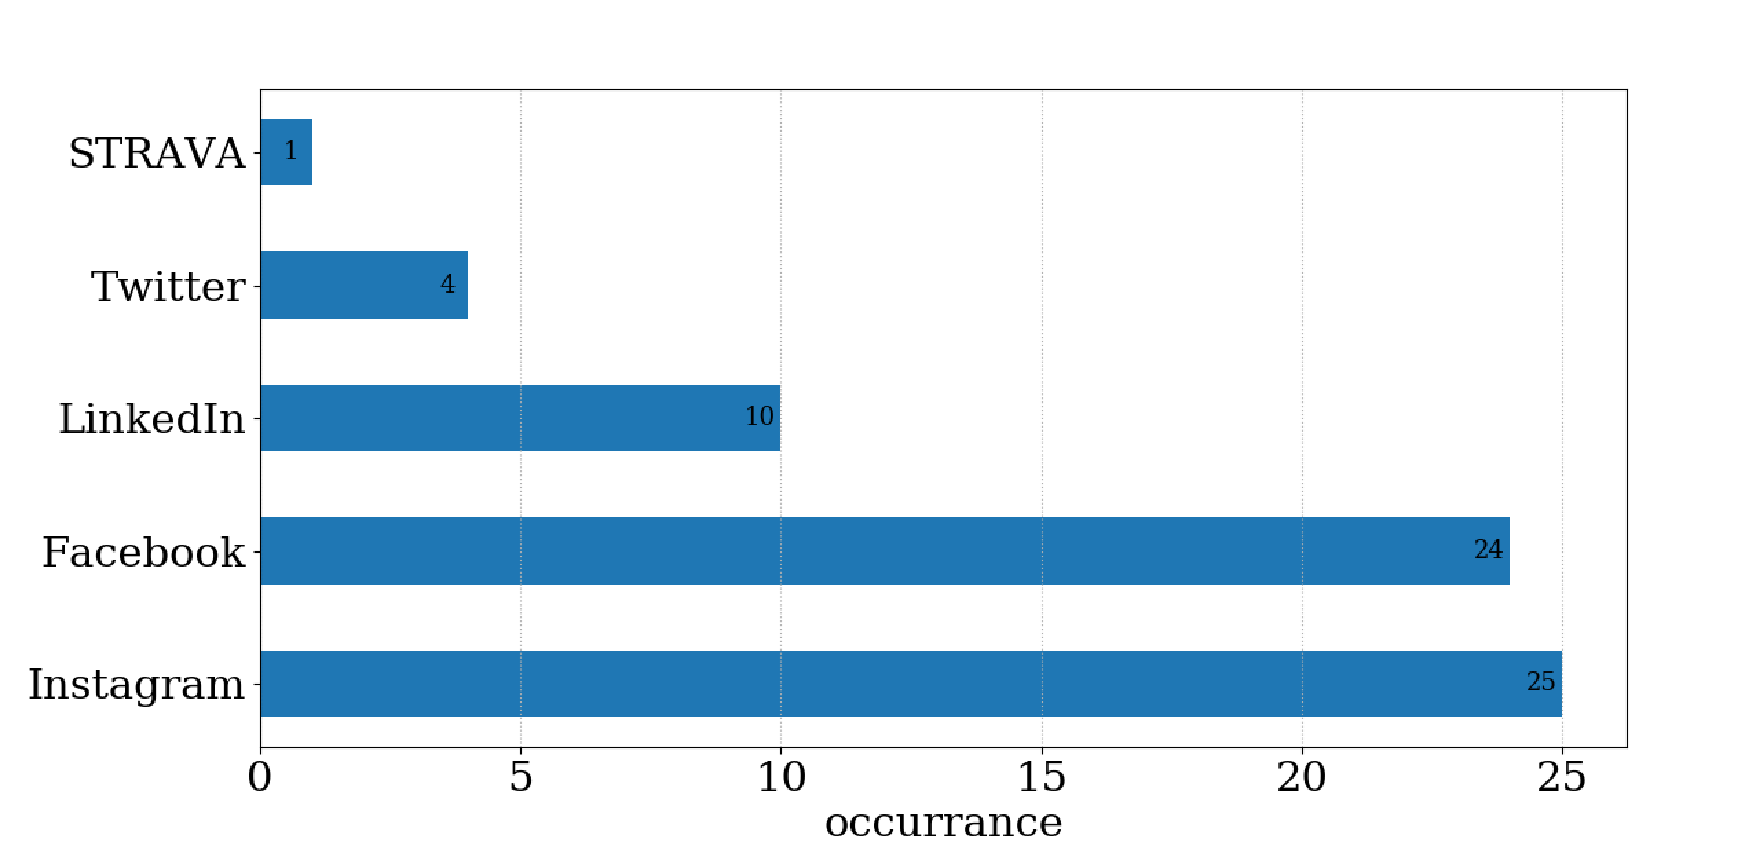
\includegraphics[width=\textwidth]{img/interview_socialmedia_bigger_font.pdf}
   \caption{Deviated social media platform popularity according to confirmed profiles of 52 interviewees}
   \label{fig:interview_SMP}
\end{figure}

\subsubsection{Relationship between age and social media presence}
Insight on dominantly represented ages groups in social media data can be drawn from figure \ref{fig:interview_age_SMP}. According to the 52 conducted interviews are the most active people on social media platforms between the age of 21 and 30 (red bars indicating participation). The age group of 61 to 100 on the other hand has not one recorded social media user. The average age of all interviewees lies at 44, the one for social media users at 33 and at 64 for non social media users. The red and blue line in figure \ref{fig:interview_age_SMP} represent the linear regression lines of the corresponding datasets. Their intersection at roughly age 50 indicates the transition between social media platform usage and absence. Instagram and Facebook make out the biggest share of these records as already seen in figure \ref{fig:interview_SMP}.

\begin{figure}[h!]
   \centering
   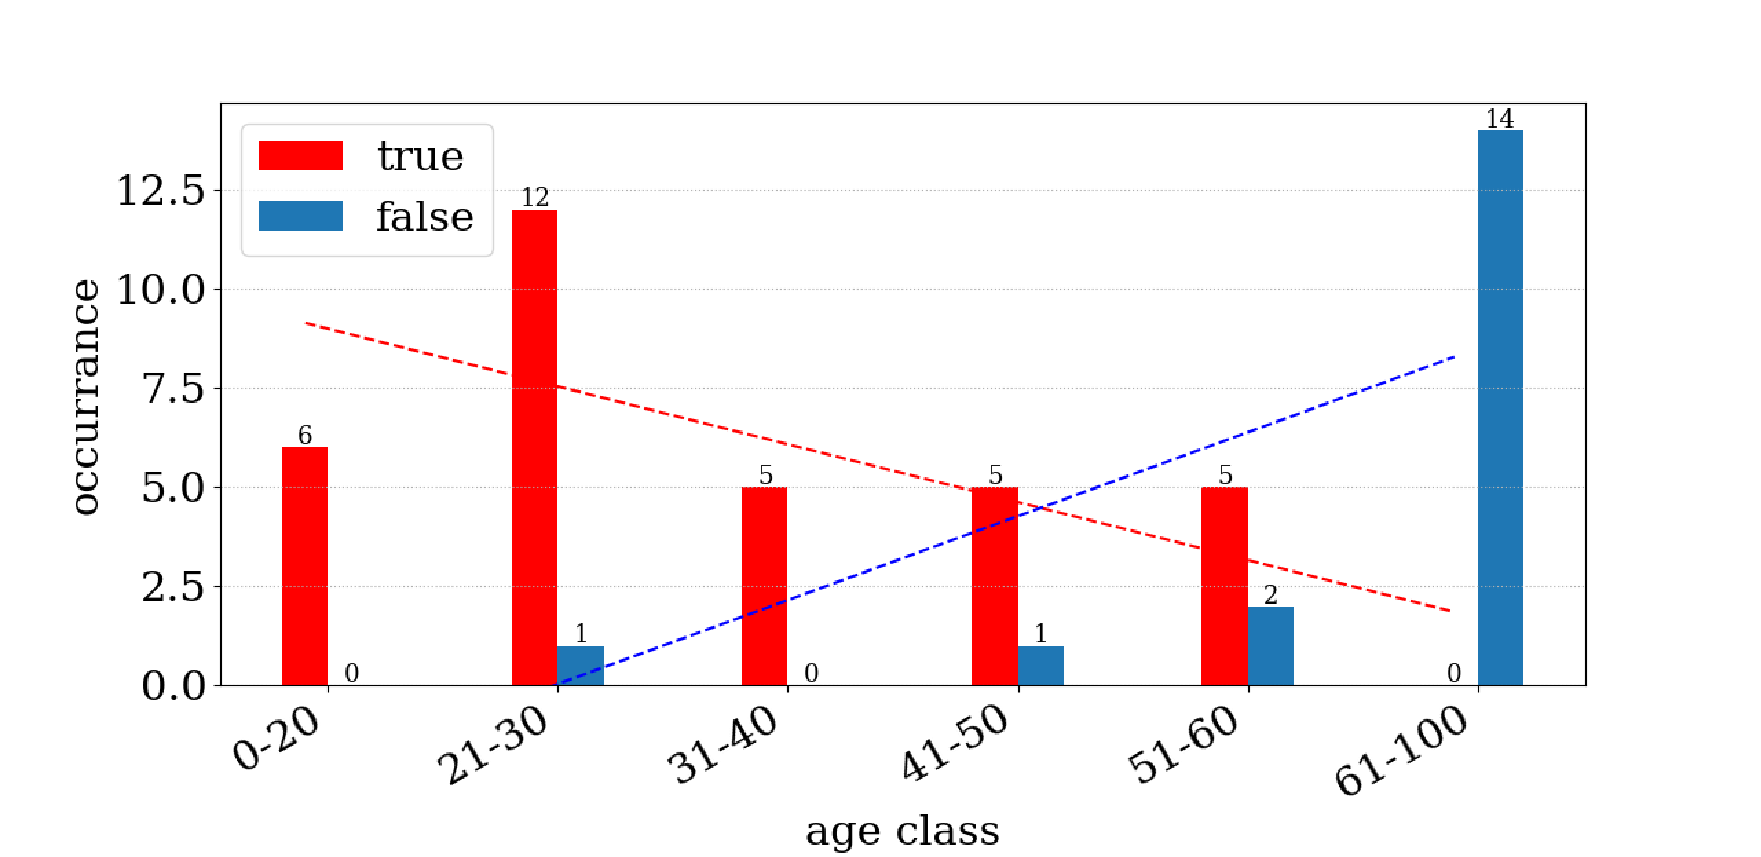
\includegraphics[width=\textwidth]{img/interview_socialmedia_age_bigger_font.pdf}
   \caption{Share per age class of social media users (true) and the once that do not use it (false). The red and blue line represent the linear regression of their corresponding dataset.}
   \label{fig:interview_age_SMP}
\end{figure}

\section{Spatial distribution of model predicted NBRAs} \label{results_spatial_dist_model_NBRA}
This section will present the maps which resulted from the M2 NBRA-predictions on both Instagram and Flickr media objects from the Canton of Zug. The maps in figure \ref{fig:map_cluster_1} and figure \ref{fig:map_cluster_2} show the NBRAs spatial distribution in parallel comparison between the two social media platforms. The amount of M2 predictions per classification and social media platform are listed in table \ref{tab:amount_class_NBRAs} as well as in the maps themselves as \textit{feature count}.

\begin{table}[h!]
\begin{center}
\caption{Amounts of M2 classified media objects that contain NBRAs}\vspace{1ex}
\label{tab:amount_class_NBRAs}
\begin{tabular}{cccc}\hline
Class & Instagram & Flickr & Total\\ \hline
Hiking & 231 & 126 & 357\\
Walking & 265 & 55 & 320\\
Dog walking & 143 & 16 & 159\\
Biking & 95 & 51 & 146\\
Jogging & 85 & 19 & 104\\
Horse riding & 37 & 6 & 43\\
Picnic & 23 & 6 & 29\\
 & & & \\
None & 10'898 & 3'511 & 14'409\\
\hline
\end{tabular}
\end{center}
\end{table}

As mentioned in section \ref{instagram_location_tag} Instagram locations can be user generated and are often general descriptions of the area at hand. This results in media objects being snapped to the same point on the map which leads to a lower spatial resolution. For further illustration a comparison between the two social media platforms in regards to location numbers is made:
There are \textbf{152} unique Instagram locations of which the top three are named 'Zug' with 1'970, 'Canton of Zug' with 1'590 and 'lake Zug' with 400 associated media objects.
The processed Flickr dataset on the other hand consists of \textbf{1'144} unique locations of which the top three are named 'Baarerstrasse 12' with 112, 'Bahnhofsplatz' with 84 and 'Landsgemeindeplatz' with 69 associated media objects. This additional geo-information in form of an address is not provided by the Flickr API by default but rather through the Google Geocoding API as stated in section \ref{geocoding_api}. \\
One has to keep in mind that the processed Flickr dataset holds only roughly a third of the media objects compared to the processed Instagram dataset in the area of interest while possessing 7.5 times as many unique locations. 

\begin{figure}[h!]
   \centering
   \includegraphics[width=\textwidth,height=\textheight,keepaspectratio]{img/map_cluster_1.pdf}
   \caption{Part 1 - Spatial NBRA-occurrences in the Canton of Zug based on M2 predictions which were conducted on text strings containing processed text-data and image labels from the Instagram / Flickr media objects.}
   \label{fig:map_cluster_1}
\end{figure}

\begin{figure}[h!]
   \centering
   \includegraphics[width=\textwidth,height=\textheight,keepaspectratio]{img/map_cluster_2.pdf}
   \caption{Part 2 - Spatial NBRA-occurrences in the Canton of Zug based on M2 predictions which were conducted on text strings containing processed text-data and image labels from the Instagram / Flickr media objects.}
   \label{fig:map_cluster_2}
\end{figure}

\subsection{Comparison to ground truth} \label{results_comp_ground_truth}
A quantitative comparison of the inferred ranking of recreational activity occurrences between the passive observation and the social media data was performed (see table \ref{tab:compare_ranking}). Interview data to recreational activities were neglected since they are considered to be a subset of the comprehensive passive observation. The Spearman's Rank-Order Correlation revealed a $\rho$=0.4 regarding the passive observation ranking compared to Instagram as well as Instagram plus Flickr ranking. Considering detected NBRAs in Flickr alone matches the ranking of the passive observation entirely ($\rho$=1). \\

\begin{table}[h!]
\begin{center}
\caption{Recreational activity ranking of the passive observation summed up over all three ground truth locations (see table \ref{fig:passive_observation}) and the social media data (see table \ref{tab:amount_class_NBRAs}). 'Walking' and 'hiking' were merged for Instagram and Flickr since the ground truth data did not differentiate between the two classes. Also, the classes 'horse riding' and 'picnic' are not included since they were not witnessed during the passive observation.}\vspace{1ex}
\label{tab:compare_ranking}
\begin{tabular}{ccccc}\hline
\textbf{\large{Ranking}}  & & $\rho$=0.4 & $\rho$=1 & $\rho$=0.4\\
Activity & Passive observation & Instagram & Flickr & Together\footnotemark\\ \hline
Walking/Hiking & 1 & 1 & 1 & 1\\
Biking & 2 & 3 & 2 & 3 \\
Jogging & 3 & 4 & 3 & 4\\
Dog walking & 4 & 2 & 4 & 2 \\
\hline
\end{tabular}
\end{center}
\end{table}
\footnotetext{Instagram plus Flickr}

Additionally, the modelled output of M2 (see maps in figure \ref{fig:map_cluster_1} and figure \ref{fig:map_cluster_2}) was visually compared to the ground truth visible in figure \ref{fig:passive_observation} and figure \ref{fig:interview_activities} to further evaluate the model's plausibility.

\paragraph*{Biking}
The model predicts a strong occurrence of biking in the area of 'R\"ossliwiese' where the ground truthing consisting of the passive observation and the interviews did not record a single sighting.\\
In the area of 'Schattenw\"aldli' and 'B\"uggli' the ground truth recorded a moderate occurrence of (mountain-)bikers which were not registered by the model. 

\paragraph*{Hiking}
'Schattenw\"aldli' is according to the interviews the only location of the three where the NBRA 'hiking' is performed. Also the model shows a strong signal of 'hiking' in the mountainous region. Contradicting are as 'hiking' classified media objects located in the urban area of the city of Zug.

\paragraph*{Jogging}
The maps as well as the ground truth show moderate congruent signals in all three locations.

\paragraph*{Walking}
M2 records a predominant signal in the urban areas over the mountainous areas. Especially the lake side is strongly represented which coincides with the interviewee given motivation 'lake' listed in figure \ref{fig:interview_visitation_motivation} as well as with the high recorded interview 'walking' frequency in the locations 'Br\"uggli' and 'R\"ossliwiese' visible in figure \ref{fig:interview_activities}. Flickr recorded one obvious false occurrence of 'walking' on the lake of Zug which resembles a media object with the title "walk on water" of a stand-up paddler.

\paragraph*{Picnic}
The ground truth does not yield any information on that classification.

\paragraph*{Dog walking}
The recreational activity 'dog walking' is according to the ground truth performed in all three locations in a comparably low frequency similar to 'jogging'. The M2 Instagram-data shows a signal densification in the urban area of the city of Zug whereas the Flickr-data shows a homogeneous distribution without any clear hot-spots.

\paragraph*{Horse riding}
The ground truth does not yield any information on that classification.

\paragraph*{None} The M2 'None' classification signal shows as expected a homogeneous distribution (especially the Flickr-data with the higher spatial resolution) without any visible patterns. Because non-NBRAs were not actively recorded during the ground truthing a direct comparison cannot be made.

\paragraph*{Summary}
Essentially predicted the model spatial patterns which coincide with the available ground truth data. An exception is the classification 'hiking' which shows discrepancy and overlaps with the classification 'walking' which will be addressed in the section \ref{discussion_rq2} of the \nameref{discussion}.

\subsection{Comparison to Foursquare}
The platform Foursquare holds records of categorised infrastructure (venues). The map in figure \ref{fig:map_foursquare_comparison} visualises 378 Foursquare venues of the category \textit{Outdoor \& Recreation} in relation to the M2 predicted NBRA-occurrences in the Instagram and Flickr dataset of the Canton of Zug.\\
For reasons of time a spatial similarity analysis between the datasets could not be conducted. Instead a visual evaluation shall give insight on the spatial concordance. The NBRA-types were not analysed individually due to the considerable overlap in supporting infrastructure between them. \\
The map shows a plausible densification of venues in or near urban areas. The occurrences of NBRAs and venues seem to match spatially quite well which suggests that the supporting infrastructure is already efficiently allocated to fit the peoples recreational needs. This claim has to be further analysed with an appropriate statistical evaluation. \\
The Foursquare dataset in conjunction with the modelled NBRA occurrences shall moreover give agencies a tool to plan the allocation of sport and recreation related infrastructure in case of rezoning or land conversion.

\begin{figure}[h!]
   \centering
   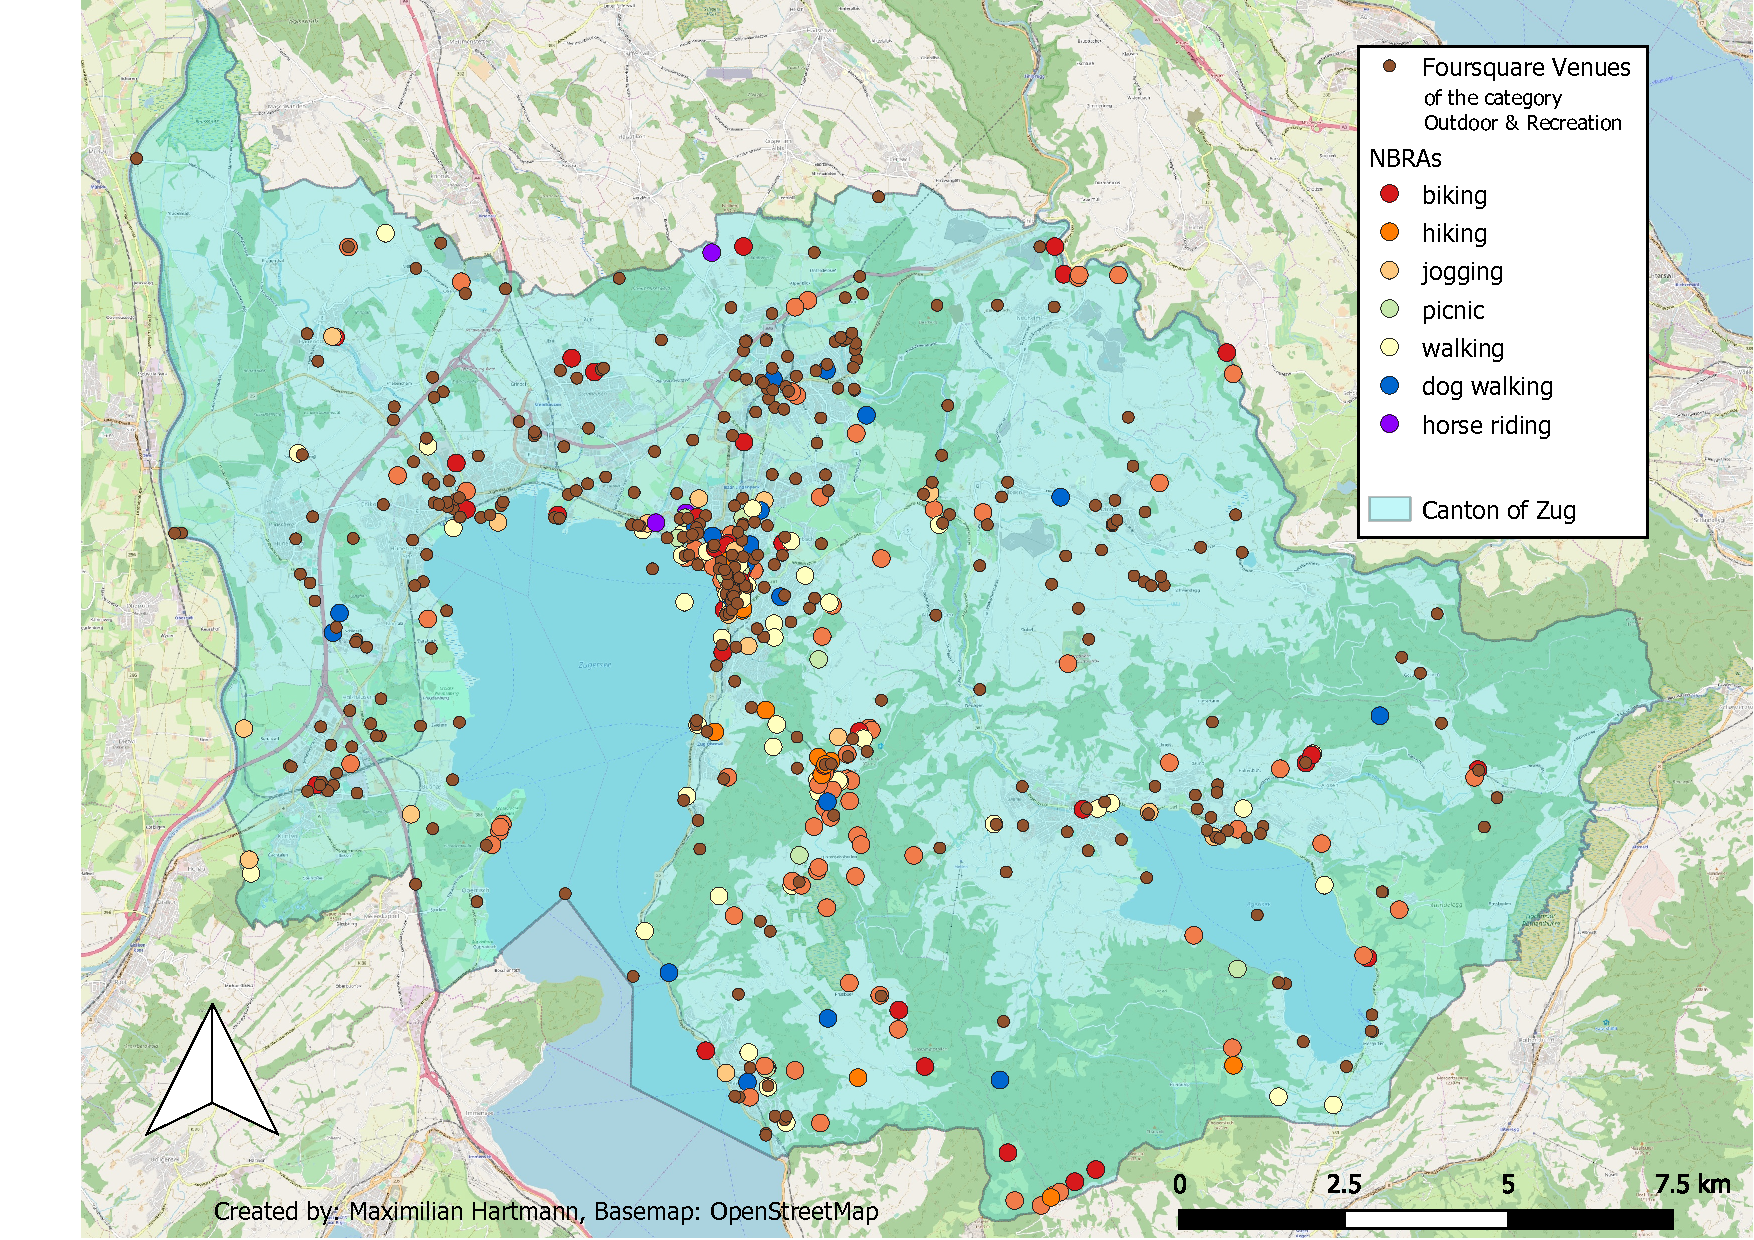
\includegraphics[width=\textwidth,height=\textheight,keepaspectratio]{img/foursquare_comparison_cropped.pdf}
   \caption{Locations of all 378 Foursquare venues of the category \textit{Outdoor \& Recreation} in relation to the M2 predicted spatial NBRA-occurrence of the social media platforms Instagram and Flickr.}
   \label{fig:map_foursquare_comparison}
\end{figure}


